% Presentation: Performance Engineering, group 11 -- CloverLeaf on HAICGU
% Build: make  (latexmk -pdf main.tex). Target: 10 min talk + 5 min questions.
\documentclass[aspectratio=169,10pt]{beamer}
\usetheme{RUG}

\usepackage[utf8]{inputenc}
\usepackage{amsmath}
\usepackage{booktabs}
\usepackage{graphicx}
\usepackage{listings}

\lstset{basicstyle=\ttfamily\tiny, columns=fullflexible, keepspaces=true, breaklines=true,
  language=C, commentstyle=\color{ruggrey}, keywordstyle=\color{rugdark}, stringstyle=\color{rugdark},
  aboveskip=2pt, belowskip=2pt, xleftmargin=0.2em}
\usetikzlibrary{shapes.geometric,arrows.meta,positioning,calc}
\tikzset{
  every picture/.style={font=\scriptsize, >={Stealth[length=4pt]}},
  loop/.style={draw=rugdark, thick, rounded corners=5pt, fill=ruglight, minimum height=0.55cm, minimum width=1.3cm, align=center, inner sep=2pt},
  arr/.style={cylinder, shape border rotate=90, aspect=0.1, draw=rugdark, fill=white, minimum width=1.0cm, minimum height=0.4cm, align=center, inner xsep=5pt, inner ysep=1.5pt},
  reg/.style={circle, draw=rugred, thick, fill=white, minimum size=0.45cm, inner sep=1pt, align=center},
  fname/.style={draw=rugdark, fill=white, font=\ttfamily\scriptsize, inner sep=2pt, minimum height=0.4cm, minimum width=1.1cm},
  save/.style={font=\tiny\bfseries, text=rugred, align=center},
  dead/.style={draw=rugred, dashed, text=rugred, fill=white},
  flow/.style={->, line width=1.4pt, ruggrey},
  data/.style={->, thin, rugdark},
  gone/.style={->, thin, rugred, dashed},
  lbl/.style={font=\tiny, text=ruggrey, align=center},
  tag/.style={font=\tiny\bfseries, text=rugred, anchor=south west, inner sep=0pt},
}
\newcommand{\kernel}[1]{\texttt{#1}}
\newcommand{\GBs}{\,GB/s}
\newcommand{\good}[1]{\textcolor{rugred}{\textbf{#1}}}

\title{Analysis and Optimisation of CloverLeaf\\on a Kunpeng 920 Node}
\subtitle{Performance Engineering, Group 11}
\author{Jort Oosterveld \and Sergiu-Adrian Preda}
\institute{Faculty of Science and Engineering, University of Groningen}
\date{October 2026}

\begin{document}

\begin{frame}[plain,noframenumbering,t]
  \titlepage
\end{frame}
\note{0:00. One sentence: we took the C kernels of CloverLeaf, found they were already at the memory
  ceiling, and made them 1.37x faster by moving fewer bytes.}

% ======================================================================
\section{Baseline}
% ======================================================================

\begin{frame}{The application and the machine}
  \begin{columns}[T]
    \begin{column}{0.5\textwidth}
      \textbf{CloverLeaf (reference, MPI + OpenMP)}
      \begin{itemize}
        \item Fluid dynamics simulator
        \item Large vectors, many nested loops
        \item Forces computed for each cell every timestep
        \item Compute-heavy \emph{kernels}, both FORTRAN and C implementations
        \item We focus on C only, FORTRAN as reference
        \item benchmark \textbf{bm3840}: $3840^2$ cells, 87 steps, $\approx$25 arrays of 118\,MB $\approx$3\,GB working set
      \end{itemize}
    \end{column}
    \begin{column}{0.5\textwidth}
      \textbf{HAICGU node}
      \begin{itemize}
        \item 2$\times$ Kunpeng 920 (ARMv8, 2.6\,GHz): 128 cores, 4 NUMA domains
        \item 16 channels DDR4-2666, 128\,GB, L3 2$\times$64\,MB
        \item GCC 14.1, OpenMPI 5.0, PAPI 7.1, Linux \texttt{perf}
        \item \texttt{-O3 -march=native -funroll-loops -fopenmp}
        \item layout ``$r\times t$'': $r$ ranks $\times$ $t$ threads, one thread per core, ranks pinned
      \end{itemize}
    \end{column}
  \end{columns}
  \vspace{0.4cm}
  \textbf{Research question:} how far is the baseline from what the hardware allows, and what does it take to close the gap?
\end{frame}
\note{0:30. Working set is 25x the L3: every loop nest streams its arrays from DRAM.}

\begin{frame}{Methodology: three independent sources, one convention}
  \begin{columns}[T]
    \begin{column}{0.55\textwidth}
      \begin{enumerate}
        \item CloverLeaf's own profiler: wall clock per phase
        \item PAPI per kernel (\texttt{papi\_prof}, one event set per thread): IPC, instruction mix, stalls
        \item Linux \texttt{perf} and the DDR-controller PMU: \textbf{bytes that cross the memory interface}, read around every run
      \end{enumerate}
      \vspace{0.3cm}
      \textbf{Protocol.} 5 repetitions, median and min--max, every one under the DDR counters: time and bytes from the same run. All bandwidths are \emph{hardware bytes} / wall clock, for STREAM and for the application alike.
    \end{column}
    \begin{column}{0.45\textwidth}
      \begin{block}{Checks of the tools}
        \begin{itemize}
          \item PAPI build costs $<$1\,\%; kernel times add up to the wall clock within 1\,\%
          \item DDR counters calibrated on STREAM: 32\,B per count, no read-for-ownership on streaming stores
          \item NUMA page distribution is fair, busiest DDR controller group has a mean of $1.00$
        \end{itemize}
      \end{block}
      \begin{block}{Correctness gate}
        \texttt{PASSED} on bm3840; deviation of the long deck \texttt{clover\_bm.in} reproduced to $10^{-6}$\,\%
      \end{block}
    \end{column}
  \end{columns}
\end{frame}
\note{1:30. The key convention: hardware bytes, not model bytes, for every bandwidth number.}

\begin{frame}{Ceilings, byte model and roofline}
  \begin{columns}[T]
    \begin{column}{0.4\textwidth}
      \small
      \textbf{Measured ceilings}
      \begin{itemize}
        \item STREAM triad, 128 threads: \textbf{266.5\GBs} hardware bytes
        \item FMA peak \textbf{1330\,GFLOP/s}: ridge at \textbf{5\,flop/B}
      \end{itemize}
      \vspace{0.2cm}
      \textbf{Analytic byte model} (arrays read and written per loop nest, write-allocate charged)
      \begin{itemize}
        \item 451\,flop, 2186\,B per cell and step: \textbf{0.21\,flop/B}
        \item predicts 2.80\,TB for bm3840; measured \textbf{2.83\,TB} ($+1$\,\%)
        \item reads $= 1.34\times$ demand: the C stores pay a read-for-ownership
      \end{itemize}
    \end{column}
    \begin{column}{0.6\textwidth}
      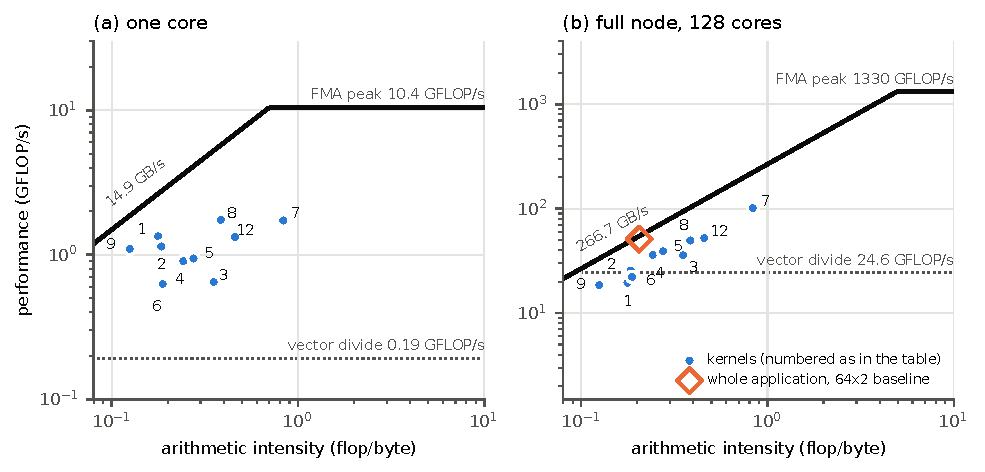
\includegraphics[width=0.96\textwidth]{figures/fig_roofline.pdf}
    \end{column}
  \end{columns}
\end{frame}
\note{3:30. Every kernel sits at 0.13-0.83 flop/B, far left of the ridge. The model is validated by the counters to 1 percent, so we can trust it to predict changes.}

\begin{frame}{Where the time goes}
  \begin{columns}[T]
    \begin{column}{0.57\textwidth}
      \footnotesize
      \begin{tabular}{lrrrr}
        \toprule
        kernel & \multicolumn{2}{c}{time share (\%)} & IPC & stall (\%) \\
               & 1 core & 128 cores & 64$\times$2 & 64$\times$2 \\
        \midrule
        \kernel{advec\_mom}  & 28.6 & \good{44.0} & 0.27 & 91 \\
        \kernel{advec\_cell} & 19.4 & \good{19.4} & 0.28 & 91 \\
        \kernel{pdv} (2 calls) & 17.6 &  9.6 & 0.21 & 92 \\
        \kernel{calc\_dt}    & 11.8 &  4.8 & 0.50 & 81 \\
        \kernel{ideal\_gas}  &  7.4 &  4.7 & 0.31 & 87 \\
        \kernel{viscosity}   &  5.7 &  2.2 & 0.99 & 62 \\
        \kernel{accelerate}  &  5.2 &  4.1 & 0.27 & 91 \\
        \kernel{reset} + \kernel{revert} & 1.6 & 4.5 & 0.10 & 96 \\
        other (3)            &  2.7 &  6.7 & -- & -- \\
        \bottomrule
      \end{tabular}
      \vspace{0.2cm}

      \scriptsize bm3840, PAPI; 128 cores $=1\times128$; stall = back-end stall cycles
    \end{column}
    \begin{column}{0.43\textwidth}
      \begin{itemize}
        \item advection $=$ 63\,\% of the node-level time; \kernel{advec\_mom} scales worst ($14\times$ on 128 cores)
        \item at 64$\times$2: IPC 0.1--0.5, \textbf{81--96\,\% back-end stalls}: the cores wait for memory
        \item \kernel{calc\_dt}, \kernel{ideal\_gas}, \kernel{viscosity} run \emph{scalar}: \texttt{sqrt} stays a libm call without \texttt{-fno-math-errno}
        \item advection upwind loops: data-dependent indices, only 12--16\,\% vector instructions
        \item 12.5\,\% of all cycles in the OpenMP barrier (one per worksharing loop)
      \end{itemize}
    \end{column}
  \end{columns}
\end{frame}

\begin{frame}{Baseline}
  \begin{columns}[T]
    \begin{column}{0.55\textwidth}
      \footnotesize
      \begin{tabular}{llrrr}
        \toprule
        kernels & layout & wall (s) & TB & \% of roof \\
        \midrule
        C & \textbf{64$\times$2} & \textbf{11.32} & 2.83 & \textbf{94} \\
        C & 32$\times$4  & 11.46 & 2.79 & 91 \\
        C & 128$\times$1 & 11.66 & 2.95 & 95 \\
        C & 4$\times$32  & 13.00 & 2.87 & 83 \\
        C & 1$\times$128 & 26.91 & 2.99 & 42 \\
        C & 1$\times$128, THP off & 13.31 & 2.83 & 80 \\
        \midrule
        Fortran & 64$\times$2 & 9.33 & \textbf{2.36} & 95 \\
        \bottomrule
      \end{tabular}
      \vspace{0.2cm}

      \scriptsize On the bm3840 test set, roof $=$ 266.5\GBs{}
      \vspace{0.1cm}

      \normalsize
      \begin{alertblock}{Finding}
        Memory performance already optimized, further gain has to come from \textbf{moving fewer bytes}, like the FORTRAN kernel.
      \end{alertblock}
    \end{column}
    \begin{column}{0.45\textwidth}
      \begin{itemize}
        \item baseline 64$\times$2: 250\GBs{} over the whole run, start-up included: \textbf{94\,\% of the hardware ceiling}
        \item time floor for memory: $2.83\,\text{TB} / 266.5\GBs = $ \textbf{10.6\,s}. Baseline is close to maximum memory performance.
        \item only 1$\times$128 cares about THP: first touch puts whole arrays on one NUMA domain ($1.66\times$ imbalance)
        \item Fortran is 18\,\% faster, because it moves \emph{fewer bytes}.
      \end{itemize}
    \end{column}
  \end{columns}
\end{frame}
\note{Remove THP if time constraint}
\note{4:30. This is the pivot of the talk. Vectorising, fewer barriers, flags: none of it can pay until the bytes shrink.}

% ======================================================================
\section{Kernel improvements}
% ======================================================================

\begin{frame}{Plan: five byte reductions, predicted with the byte model}
  \footnotesize
  \begin{tabular}{p{8.2cm}rrr}
    \toprule
    change & DRAM bytes & cumulative & floor (s) \\
    \midrule
    (1) \kernel{advec\_mom}: direction-only helper loops once per sweep, not once per velocity component & $-12.8$\,\% & $-12.8$\,\% & 9.2 \\
    (2) \kernel{advec\_cell}: four temporaries in registers instead of four full-mesh arrays & $-5.9$\,\% & $-18.7$\,\% & 9.9 \\
    (3) dead stores \texttt{post\_vol} / \texttt{pre\_vol}: written over the haloed grid, never read & $-4.4$\,\% & $-21.6$\,\% & 10.1 \\
    (4) Reset / Revert: swap the field allocations instead of copying 118\,MB per field & $-6.6$\,\% & $-28.2$\,\% & 9.8 \\
    (5) \kernel{calc\_dt}: fuse the min reduction into the compute loop & $-1.1$\,\% & \good{$-29.3$\,\%} & \good{7.4} \\
    \midrule
    (6) streaming stores (no read-for-ownership), upper bound & $-22.8$\,\% & $-41.4$\,\% & -- \\
    \bottomrule
  \end{tabular}
  \vspace{0.15cm}
  \normalsize
  \begin{itemize}
    \item selection: the three kernels with the largest gain in the model; (3) and (5) fell out while reading the code
    \item every change is an edit of the model's loop table, so prediction and measurement share one convention; time-only items (\texttt{nowait}, \texttt{-fno-math-errno}, branch-free upwind loop) come after the bytes
  \end{itemize}
\end{frame}
\note{5:30. Floor = predicted bytes / 266.5 GB/s.}

% Schematic data-flow views of the byte reductions (presentation only; not in the report).
% Shapes: rounded box = loop nest over the grid, cylinder = full-mesh array in DRAM (118 MB),
% circle = register / scalar; grey arrow = program order, thin arrow = bytes through DRAM,
% red dashed = traffic and work that the change removes.

\newcommand{\schemalegend}{%
  \begin{tikzpicture}[baseline=(l1.base)]
    \node[loop, minimum width=0.9cm, minimum height=0.4cm] (l1) {loop nest};
    \node[arr] (l2) at (2.0,0) {array in DRAM};
    \node[reg] (l3) at (3.5,0) {reg};
    \node[fname] (l4) at (4.6,0) {name};
    \draw[flow] (5.4,0) -- (6.0,0) node[lbl, right] {program order};
    \draw[data] (7.6,0) -- (8.2,0) node[lbl, right] {bytes through DRAM};
    \draw[gone] (10.7,0) -- (11.3,0) node[lbl, right] {removed by the change};
  \end{tikzpicture}}

\begin{frame}{Data flow (1/2): work that was done twice}
  \begin{columns}[T]
    % ---------------------------------------------------------- (1) advec_mom
    \begin{column}{0.56\textwidth}
      \textbf{(1) \kernel{advec\_mom}: helper loops once per sweep}
      \par\vspace{0.1cm}
      \begin{tikzpicture}
        \node[tag] at (-0.65,0.42) {before};
        \node[loop] (p1) at (0,0)    {prep\\4 loops};
        \node[loop] (x)  at (1.55,0) {\kernel{xvel}\\loop};
        \node[loop,dead] (p2) at (3.1,0)  {prep\\4 loops};
        \node[loop] (y)  at (4.65,0) {\kernel{yvel}\\loop};
        \draw[flow] (p1) -- (x); \draw[flow] (x) -- (p2); \draw[flow] (p2) -- (y);
        \node[arr] (A) at (0.8,-0.95)  {8 node arrays};
        \node[arr,dead] (B) at (3.9,-0.95) {the same 8, rebuilt};
        \draw[data] (p1.south) -- (A.north);
        \draw[data] (A.north) -- (x.south);
        \draw[gone] (p2.south) -- (B.north);
        \draw[gone] (B.north) -- (y.south);
        \node[lbl, anchor=west] at (5.3,-0.95) {full mesh, streamed\\twice per sweep};
      \end{tikzpicture}
      \par\vspace{0.15cm}
      \begin{tikzpicture}
        \node[tag] at (-0.65,0.42) {after};
        \node[loop] (p1) at (0,0)    {prep\\4 loops};
        \node[loop] (x)  at (1.55,0) {\kernel{xvel}\\loop};
        \node[loop] (y)  at (3.1,0)  {\kernel{yvel}\\loop};
        \draw[flow] (p1) -- (x); \draw[flow] (x) -- (y);
        \node[arr] (A) at (1.55,-0.95) {8 node arrays};
        \draw[data] (p1.south) -- (A.north);
        \draw[data] (A.north) -- (x.south);
        \draw[data] (A.north) -- (y.south);
        \node[lbl, anchor=west] at (2.8,-0.95) {built once per sweep,\\read by both\\velocity passes};
      \end{tikzpicture}
    \end{column}
    % ---------------------------------------------------------- (4) reset / revert
    \begin{column}{0.44\textwidth}
      \textbf{(4) Reset / Revert: swap, not copy}
      \par\vspace{0.1cm}
      \begin{tikzpicture}
        \node[tag] at (-0.65,0.45) {before};
        \node[arr]       (d1) at (0,0)   {density1};
        \node[loop,dead] (cp) at (2.0,0) {copy loop\\(\kernel{reset\_field})};
        \node[arr]       (d0) at (4.0,0) {density0};
        \draw[gone] (d1) -- (cp);
        \draw[gone] (cp) -- (d0);
        \node[lbl] at (2.0,-0.7) {$\times$4 fields, every step:\\read $+$ write $+$ read-for-ownership};
      \end{tikzpicture}
      \par\vspace{0.15cm}
      \begin{tikzpicture}
        \node[tag] at (-0.65,0.62) {after};
        \node[fname] (n1) at (0,0.35)  {density1};
        \node[fname] (n0) at (0,-0.35) {density0};
        \node[arr] (bA) at (2.9,0.35)  {buffer A (new)};
        \node[arr] (bB) at (2.9,-0.35) {buffer B (old)};
        \draw[data, dashed, ruggrey] (n1.east) -- (bA.west);
        \draw[data, dashed, ruggrey] (n0.east) -- (bB.west);
        \draw[data] (n1.east) -- (bB.west);
        \draw[data] (n0.east) -- (bA.west);
                \node[lbl] at (2.0,-0.95) {dashed: before the swap, solid: after. Three \texttt{MOVE\_ALLOC}s\\per field, no bytes move; the kernels find the field under its new name};
      \end{tikzpicture}
      \par\vspace{0.15cm}
      \scriptsize Same for the \texttt{revert} kernel, this one is skipped as well.
    \end{column}
  \end{columns}
  \vspace{0.15cm}
  \centering\schemalegend
\end{frame}
\note{9:30. Two changes that remove whole loop nests: the helper loops of advec\_mom ran once per velocity component and rebuilt the same arrays; Reset copied four fields that only needed a new name.}

\begin{frame}{Data flow (2/2): round trips through DRAM}
  \begin{columns}[T]
    % ---------------------------------------------------------- (2) advec_cell + PdV
    \begin{column}{0.5\textwidth}
      \textbf{(2) \kernel{advec\_cell}: temporaries in registers}
      \par\vspace{0.1cm}
      \begin{tikzpicture}
        \node[tag] at (-0.65,0.42) {before};
        \node[arr]      (O) at (0,0)   {density1, energy1};
        \node[loop]     (L) at (2.4,0) {sweep\\loop};
        \node[arr,dead] (T) at (5.0,0) {4 temporaries};
        \draw[data] (L.west) -- (O.east);
        \draw[gone] ([yshift=5pt]L.east) -- node[lbl, above=1pt] {store $\cdot$ RFO} ([yshift=5pt]T.west);
        \draw[gone] ([yshift=-5pt]T.west) -- node[lbl, below=1pt] {reload} ([yshift=-5pt]L.east);
      \end{tikzpicture}
      \par\vspace{0.15cm}
      \begin{tikzpicture}
        \node[tag] at (-0.65,0.42) {after};
        \node[arr]  (O) at (0,0)   {density1, energy1};
        \node[loop] (L) at (2.4,0) {sweep\\loop};
        \node[reg] (r1) at (3.9,0) {}; \node[reg] (r2) at (4.5,0) {};
        \node[reg] (r3) at (5.1,0) {}; \node[reg] (r4) at (5.7,0) {};
        \draw[data] (L.west) -- (O.east);
        \draw[data, <->] (L.east) -- (r1.west);
        \node[lbl] at (4.8,-0.55) {4 scalars per cell:\\same arithmetic, same order};
      \end{tikzpicture}
      \par\vspace{0.15cm}
      \scriptsize Same in both PdV passes: \texttt{volume\_change}, stored and reloaded in one iteration, now a scalar.
      \par\vspace{0.15cm}
      \textbf{(3) Dead stores (advec\_cell \& advec\_mom)}
      \par\vspace{0.1cm}
      \begin{tikzpicture}
        \node[tag] at (-0.65,0.5) {before};
        \node[loop]     (L) at (0,0)   {sweep 1\\loop};
        \node[arr,dead] (P) at (2.9,0) {unused\_var};
        \draw[gone] (L.east) -- node[lbl, above=1pt] {write $+$ RFO} (P.west);
        \draw[gone] (P.east) -- (4.0,0) node[lbl, anchor=west] {never read};
        \node[tag] at (5.4,0.42) {after};
        \node[lbl, anchor=west, text=rugdark, align=left] at (5.4,0) {store deleted,\\value stays\\in a register};
      \end{tikzpicture}
    \end{column}
    % ---------------------------------------------------------- (5) calc_dt
    \begin{column}{0.5\textwidth}
      \textbf{(5) \kernel{calc\_dt}: fused reduction}
      \par\vspace{0.1cm}
      \begin{tikzpicture}
        \node[tag] at (-0.65,0.7) {before};
        \node[loop]     (A)  at (0,0)   {per-cell\\limits};
        \node[arr,dead] (D)  at (1.8,0) {dt\_min};
        \node[loop]     (B)  at (3.6,0) {min over\\cells};
        \node[reg]      (dt) at (5.0,0) {dt};
        \draw[flow] (A.north) to[bend left=28] (B.north);
        \draw[gone] (A) -- (D);
        \draw[gone] (D) -- (B);
        \draw[data] (B) -- (dt);
        \node[lbl] at (1.8,-0.7) {one full-mesh array written,\\then read once by a second loop};
      \end{tikzpicture}
      \par\vspace{0.15cm}
      \begin{tikzpicture}
        \node[tag] at (-0.65,0.5) {after};
        \node[loop] (A)  at (0.5,0) {per-cell limits\\$+$ \texttt{min} reduction};
        \node[reg]  (dt) at (4.2,0) {dt};
        \draw[data] (A) -- node[lbl, above=2pt] {OpenMP\\\texttt{reduction(min)}} (dt);
        \node[lbl] at (1.7,-0.7) {one pass over the grid};
      \end{tikzpicture}
      \par\vspace{0.3cm}
    \end{column}
  \end{columns}
\end{frame}
\note{10:30. Three flavours of the same waste: a value stored to a full-mesh array and reloaded in the same iteration, a store nothing reads, and a reduction split into two passes over the grid.}


% ======================================================================
\section{Results}
% ======================================================================

\begin{frame}{Ladder at 64$\times$2: the wall clock follows the bytes}
  \begin{columns}[T]
    \begin{column}{0.67\textwidth}
      \footnotesize\setlength{\tabcolsep}{4pt}
      \begin{tabular}{llrrrr}
        \toprule
        build & contents & wall (s) & TB & bytes & time \\
        \midrule
        base  & baseline source                    & 11.31 & 2.83 & -- & -- \\
        flags & the two flags only                 & 11.28 & 2.85 & $+0.7$\,\% & $-0.2$\,\% \\
        cell  & flags $+$ (2) (3) (4)              &  9.92 & 2.49 & $-12.1$\,\% & $-12.3$\,\% \\
        mom   & flags $+$ (1) (3) (5)              &  9.54 & 2.41 & $-14.9$\,\% & $-15.7$\,\% \\
        opt   & all, with the flags                & 8.25 & 2.04 & $-27.8$\,\% & $-27.0$\,\% \\
        optnf & all, baseline flags                & 8.56 & 2.05 & $-27.4$\,\% & $-24.3$\,\% \\
        \textbf{pdv} & optnf $+$ PdV scalar & \textbf{8.25} & \textbf{2.01} & \good{$-28.8$\,\%} & \good{$-26.5$\,\%} \\
        \bottomrule
      \end{tabular}
      \par\vspace{0.1cm}
      \scriptsize jobs 34938, 35003 (optnf), 35016 (pdv): one node, 5 repetitions per build (spread $\le 1$\,\%), DDR counters on
    \end{column}
    \begin{column}{0.33\textwidth}
      \begin{itemize}
        \item the lines add up: $-28.8$\,\% bytes against the \textbf{$-30.8$\,\% the model predicted}
        \item every build sustains 240--252\GBs: still on the roof, so time $\propto$ bytes
        \item the flags: 0\,\% on the baseline, 3.6\,\% on the optimised kernels, and they break the gate; \textbf{pdv} is the final build
        \item \good{1.37$\times$} at 64$\times$2: 11.32\,s to 8.26\,s
      \end{itemize}
    \end{column}
  \end{columns}
\end{frame}
\note{9:00. The model predicted within two points. That is the main methodological result. opt is the flagged build; optnf drops the flags, pdv adds Sergiu's PdV scalar and is the final one. The 0.3 s the flags bought, the PdV bytes buy back.}

\begin{frame}{Every layout, every kernel}
  \begin{columns}[T]
    \begin{column}{0.42\textwidth}
      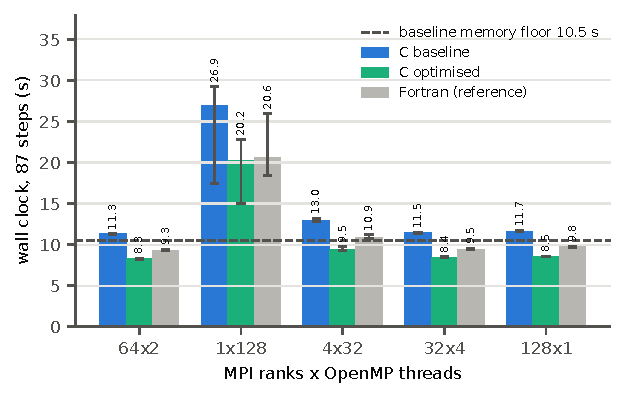
\includegraphics[width=0.9\textwidth]{figures/fig_m3_layouts.pdf}
      \begin{center}\scriptsize\setlength{\tabcolsep}{3pt}
        \begin{tabular}{lccccc}
          \toprule
          layout & 64$\times$2 & 32$\times$4 & 128$\times$1 & 4$\times$32 & 1$\times$128 \\
          speed-up & 1.37 & 1.36 & 1.36 & 1.37 & 1.33 \\
          \bottomrule
        \end{tabular}
      \end{center}
    \end{column}
    \begin{column}{0.58\textwidth}
      \footnotesize
      \begin{tabular}{lrrr}
        \toprule
        kernel & base (s) & pdv (s) & ratio \\
        \midrule
        \kernel{advec\_mom}  & 4.19 & 2.62 & \textbf{1.60} \\
        \kernel{advec\_cell} & 2.42 & 1.67 & \textbf{1.45} \\
        \kernel{pdv} (both passes) & 1.32 & 1.17 & 1.13 \\
        \kernel{calc\_dt}    & 0.66 & 0.62 & 1.05 \\
        \kernel{ideal\_gas}  & 0.58 & 0.54 & 1.06 \\
        \kernel{reset} $+$ \kernel{revert} & 0.57 & -- & gone \\
        \kernel{accel.} $+$ \kernel{flux} & 0.95 & 1.00 & 0.95 \\
        \bottomrule
      \end{tabular}
      \par\vspace{0.05cm}
      \scriptsize PAPI region times at 64$\times$2, jobs 34798 and 35017 (pdv)
      \vspace{0.05cm}

      \normalsize
      \begin{itemize}
        \item the same quarter of the traffic gone at every layout, the same speed-up
        \item optimised C is now \textbf{faster than the Fortran reference at every layout}
        \item the application moved \emph{up} the roof, not off it: 91\,\% of the ceiling, 9\,\% above the floor of its own bytes
      \end{itemize}
    \end{column}
  \end{columns}
\end{frame}
\note{9:45.}

\begin{frame}{Correctness, and what is still open}
  \begin{columns}[T]
    \begin{column}{0.5\textwidth}
      \textbf{Gate on \texttt{clover\_bm.in} ($960^2$, 2955 steps)}
      \begin{itemize}
        \item the ladder's baseline binary reproduces the archived reference (0.0057\,\%) at every layout
        \item every build with the two compiler flags, flags-only included, gives \emph{one and the same} other value (0.038\,\%): the flags alone move it (GCC's multiply-add contraction; bisect, job 34936)
        \item \textbf{optnf} (kernel changes, baseline flags) and \textbf{pdv} (optnf $+$ PdV scalar) reproduce the reference at every layout (7 of 7 each)
        \item the flags were worth 3.6\,\% on top (vectorised \texttt{sqrt} in \kernel{calc\_dt}, \kernel{ideal\_gas}): a measured trade-off, decided for reproducibility
      \end{itemize}
    \end{column}
    \begin{column}{0.5\textwidth}
      \textbf{Limitations and next steps}
      \begin{itemize}
        \item still on the bandwidth roof: 91\,\% of 266.5\GBs, floor 7.6\,s; \kernel{accelerate}, \kernel{flux\_calc}, \kernel{viscosity} untouched: the next bytes to remove
        \item read-for-ownership of the C stores: up to $-23$\,\% more bytes with explicit streaming stores
        \item \texttt{nowait} and branch-free upwind loop still open in \kernel{advec\_cell}: worth at most 9\,\%
      \end{itemize}
    \end{column}
  \end{columns}
\end{frame}
\note{10:15. The base binary reproduces the reference, the flags-only build does not, every kernel change on top of the flags gives exactly the flags value: the flags are the cause. optnf (same kernels, baseline flags) passes 7 of 7. The flags are worth 3.6 percent, in calc\_dt and ideal\_gas, and we chose the gate over them. Sergiu's bisect with contraction off shows the mechanism: FMA fusion. Sergiu's PdV scalar passed the gate too and is the final build.}

\begin{frame}{Conclusions}
  \begin{enumerate}
    \item The C kernels are memory-bound (0.2\,flop/B against a 5\,flop/B ridge) and the baseline already sustains 94\,\% of the 266.5\GBs{} hardware ceiling: \textbf{only fewer bytes can make it faster}.
    \item An analytic byte model, validated by the DDR counters to 1\,\%, predicted five changes at $-29$\,\% of the traffic, six at $-31$\,\%; measured: $-28.8$\,\%.
    \item The wall clock followed the bytes: \textbf{1.37$\times$ at 64$\times$2, 1.33--1.37$\times$ at every layout}; the optimised C build beats the Fortran reference everywhere and passes the gate.
    \item The two compiler flags are worth 3.6\,\% on the optimised kernels but break bitwise reproducibility of the reference: dropped, as a measured trade-off. The next lever is the read-for-ownership of the stores, not instruction-side work.
  \end{enumerate}
  \vspace{0.8cm}
  \begin{center}
    \Large\color{rugred} Questions?
  \end{center}
\end{frame}
\note{11:00. Stop here.}

\end{document}
